\documentclass[../main/main.tex]{subfiles}

%_______________________________________________________________________________________________________________________
\begin{document}

\section{Aproximação de Derivadas em HiGs}

\begin{frame}{Problema Modelo: Equação de Poisson}
\begin{block}{Equação de Poisson}
\[
\nabla^2 u(x, y) = f(x, y) \quad \text{em } \Omega \subset \mathbb{R}^2
\]
\end{block}

\begin{columns}[T]
\begin{column}{0.5\textwidth}
\begin{figure}
\centering
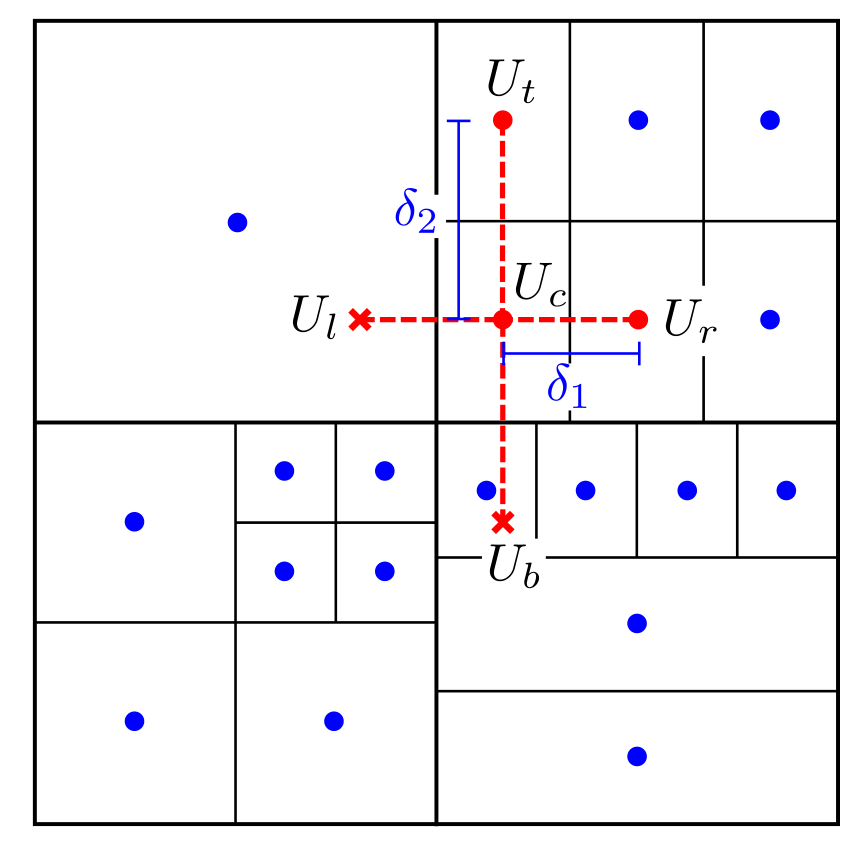
\includegraphics[width=0.8\textwidth]{imgs/figura2.png}
\caption{Estêncil FD de 2ª ordem}
\end{figure}
\end{column}
\begin{column}{0.5\textwidth}
Aproximação FD padrão:
\[
\frac{1}{\delta_1^2}(U_l - 2U_c + U_r) + \frac{1}{\delta_2^2}(U_t - 2U_c + U_b) = f_c
\]
\end{column}
\end{columns}
\end{frame}

\begin{frame}{Interpolação Meshless}
\begin{itemize}
\item Em malhas não uniformes, pontos como $U_t$ e $U_b$ não coincidem com a malha
\item Necessidade de interpolação:
\[
U_t = \sum_{k \in \mathcal{I}_t} w_k^t U_k, \quad U_b = \sum_{k \in \mathcal{I}_b} w_k^b U_k
\]
\item $\mathcal{I}_t, \mathcal{I}_b$: conjuntos de índices de vizinhos
\item $w_k^t, w_k^b$: pesos computados via MLS
\end{itemize}
\end{frame}

\begin{frame}{Aproximação Final}
\begin{block}{Sistema Linear Resultante}
\[
\frac{1}{\delta_1^2}\left(\sum_{k \in \mathcal{I}_t} w_k^t U_k - 2U_c + U_r\right) + \frac{1}{\delta_2^2}\left(U_t - 2U_c + \sum_{k \in \mathcal{I}_b} w_k^b U_k\right) = f_c
\]
\end{block}

\begin{block}{Forma Matricial}
\[
\sum_{k=1}^{N_u} A_k U_k = f_c, \quad c = 1, \ldots, N_u
\]
\[
A\mathbf{u} = \mathbf{f}
\]
\end{block}
\end{frame}

\section{Moving Least Squares (MLS)}

\begin{frame}{Fundamentos do MLS}
\begin{block}{Aproximação}
\[
U(\mathbf{x}) = \sum_{j=1}^n c_j \Phi_j(\mathbf{x})
\]
\end{block}

\begin{itemize}
\item $\Phi_j$: funções de base polinomiais
\item $c_j$: coeficientes determinados por mínimos quadrados
\item Minimização do erro ponderado:
\[
E(\mathbf{c}) = \sum_{i=1}^m \left(U(\mathbf{x}_i) - u_i\right)^2 \lambda_i(\mathbf{x})
\]
\item Pesos: $\lambda_i(\mathbf{x}) = \frac{1}{\|\mathbf{x} - \mathbf{x}_i\|_2}$
\end{itemize}
\end{frame}

\begin{frame}{Formulação Matricial}
\begin{block}{Problema de Mínimos Quadrados}
\[
E(\mathbf{c}) = \|W P \mathbf{c} - W \mathbf{u}\|_2^2
\]
\end{block}

\begin{itemize}
\item $W$: matriz diagonal de pesos
\item $P$: matriz de avaliação da base polinomial
\item Solução via decomposição QR:
\[
WP = Q \begin{bmatrix} R \\ 0 \end{bmatrix} = \begin{bmatrix} Q_\parallel & Q_\perp \end{bmatrix} \begin{bmatrix} R \\ 0 \end{bmatrix}
\]
\item Coeficientes ótimos:
\[
\mathbf{c}(\mathbf{x}) = R^{-1} Q_\parallel^T W \mathbf{u}
\]
\end{itemize}
\end{frame}

\begin{frame}{Cálculo dos Pesos de Interpolação}
\begin{block}{Pesos $w_i$}
\[
U(\mathbf{x}) = \sum_{i=1}^m w_i(\mathbf{x}) u(\mathbf{x}_i)
\]
\[
\mathbf{w} = W Q_\parallel R^{-1} \Phi(\mathbf{x})
\]
\end{block}

\begin{block}{Propriedades Importantes}
\begin{itemize}
\item Partição da unidade: $\sum_{i=1}^m w_i = 1$
\item Recuperação exata de funções de base
\item Invariância sob transformações rígidas (para polinômios completos)
\end{itemize}
\end{block}
\end{frame}

\begin{frame}{Algoritmo MLS}
\begin{block}{Algoritmo 1: Cálculo dos coeficientes $w_i$}
\begin{enumerate}
\item Dados: $\mathbf{x}_1, \ldots, \mathbf{x}_m, \mathbf{x} \in \mathbb{R}^d$, $\Phi_1, \ldots, \Phi_n$
\item Compute $W = [\delta_{ij}/\lambda_i(\mathbf{x})]$, $P = [\Phi_j(\mathbf{x}_i)]$
\item Decomposição QR de $WP \rightarrow R$ e $Q_\parallel$
\item Compute $\Phi = (\Phi_1(\mathbf{x}), \ldots, \Phi_n(\mathbf{x}))^T$
\item Resolva $R^T \mathbf{d} = \Phi$
\item Compute $\mathbf{w} = W Q_\parallel \mathbf{d}$
\end{enumerate}
\end{block}
\end{frame}

\begin{frame}{Aspectos Práticos}
\begin{itemize}
\item \textbf{Raio de interpolação}: inicialmente $3 \times \max\{\delta_1, \ldots, \delta_d\}$
\item \textbf{Adaptatividade}: aumento do raio se $R$ for singular
\item \textbf{Cache}: pesos podem ser armazenados para malhas estáticas
\item \textbf{Paralelização}: computações locais e independentes
\end{itemize}

\begin{block}{Matrizes Resultantes}
\begin{itemize}
\item Esparsas (dependendo do tamanho da vizinhança)
\item Não simétricas
\item Solucionadores iterativos: GMRES, Bi-CG
\end{itemize}
\end{block}
\end{frame}

\section{Condições de Contorno}

\begin{frame}{Condições de Contorno Dirichlet}
\begin{columns}[T]
\begin{column}{0.5\textwidth}
\begin{figure}
\centering
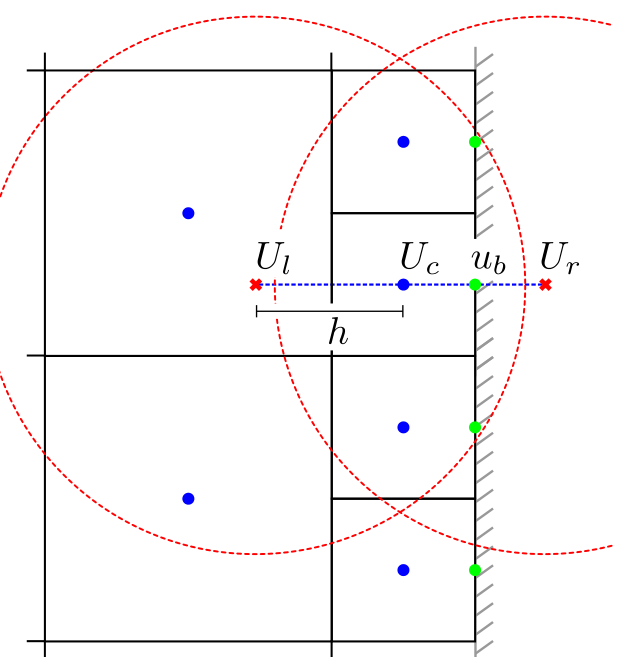
\includegraphics[width=0.9\textwidth]{imgs/figura3a.png}
\caption{Condição Dirichlet}
\end{figure}
\end{column}
\begin{column}{0.5\textwidth}
\begin{itemize}
\item Valores conhecidos nos pontos de fronteira
\item Incorporados nas interpolações MLS
\item Similar a técnicas FD padrão
\item $u_b$ imposto nos pontos verdes
\end{itemize}
\end{column}
\end{columns}
\end{frame}

\begin{frame}{Condições de Contorno Neumann}
\begin{columns}[T]
\begin{column}{0.5\textwidth}
\begin{figure}
\centering
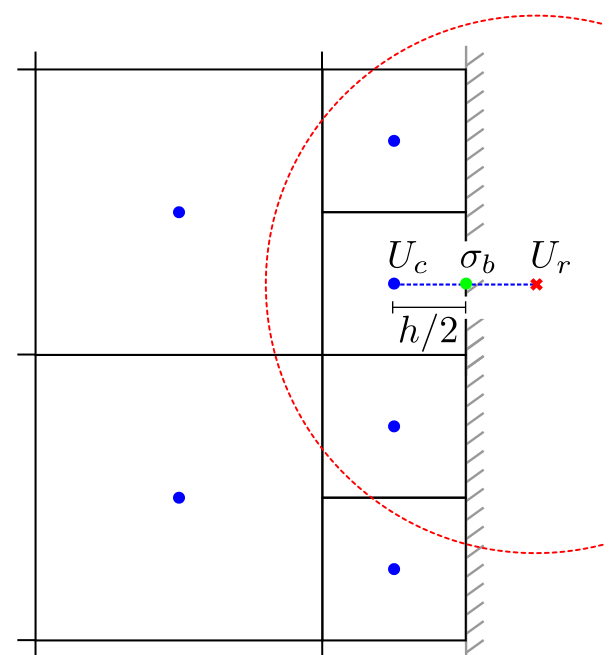
\includegraphics[width=0.9\textwidth]{imgs/figura3b.png}
\caption{Condição Neumann}
\end{figure}
\end{column}
\begin{column}{0.5\textwidth}
\begin{itemize}
\item $\frac{\partial u}{\partial x} = \sigma_b$ na fronteira direita
\item Discretização por diferenças finitas:
\[
U_r = U_c + h\sigma_b
\]
\item $h$: tamanho das células menores
\item Modificação do estêncil em $U_c$
\end{itemize}
\end{column}
\end{columns}
\end{frame}

\section{Verificação Numérica}

\begin{frame}{Verificação: Equação de Poisson em HiG Geral}
\begin{itemize}
\item Domínio: $\Omega = [-1, 1]^2$
\item Malha geral com "hanging nodes"
\item Solução analítica: $u(x, y) = \sin(x)\cos(y)$
\item Polinômios de 2º grau para MLS
\item Refinamento uniforme das células
\end{itemize}

\begin{figure}
\centering
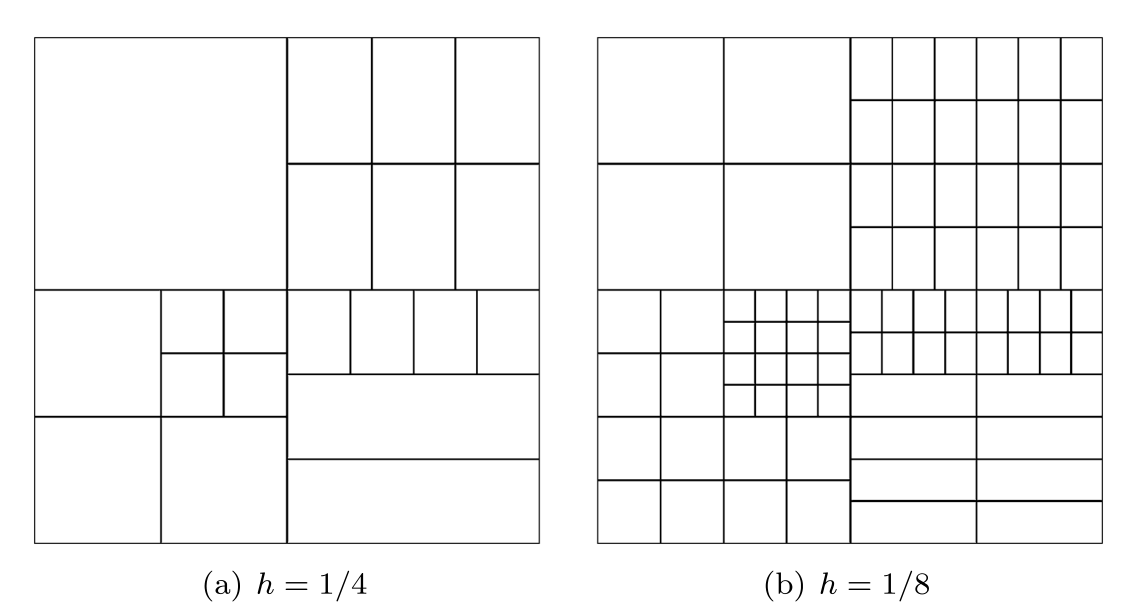
\includegraphics[width=0.7\textwidth]{imgs/figura4.png}
\caption{Malhas refinadas: (a) $h=1/4$, (b) $h=1/8$}
\end{figure}
\end{frame}

\begin{frame}{Resultados de Convergência - Poisson}
\begin{table}
\centering
\caption{Erros e ordem de convergência para Poisson em HiG geral}
\begin{tabular}{cccccc}
\toprule
$h$ & $\|u-u_h\|_{L_2}$ & EOC & $\|u-u_h\|_{L_\infty}$ & EOC \\
\midrule
1/4 & 1.29e-01 & -- & 1.21e-01 & -- \\
1/8 & 7.06e-03 & 4.1 & 8.66e-03 & 3.8 \\
1/16 & 1.30e-03 & 3.3 & 1.66e-03 & 3.1 \\
1/32 & 2.32e-04 & 3.0 & 3.14e-04 & 2.9 \\
\bottomrule
\end{tabular}
\end{table}

\begin{itemize}
\item Convergência de 2ª ordem confirmada
\item Robustez mesmo com muitas interfaces não coincidentes
\item Uso intensivo de interpolações em todas as interfaces
\end{itemize}
\end{frame}

\section{Convergência em Malhas Non-Graded}

\begin{frame}{Malhas Non-Graded Quadtree}
\begin{columns}[T]
\begin{column}{0.5\textwidth}
\begin{itemize}
\item Domínio: $[0, \pi]^2$
\item Solução exata: $u(x, y) = e^{-x-y}$
\item Condições Dirichlet
\item Teste de convergência em malha não-graded
\item Comparação com Min et al. [14] e Batty [12]
\end{itemize}
\end{column}
\begin{column}{0.5\textwidth}
\begin{figure}
\centering
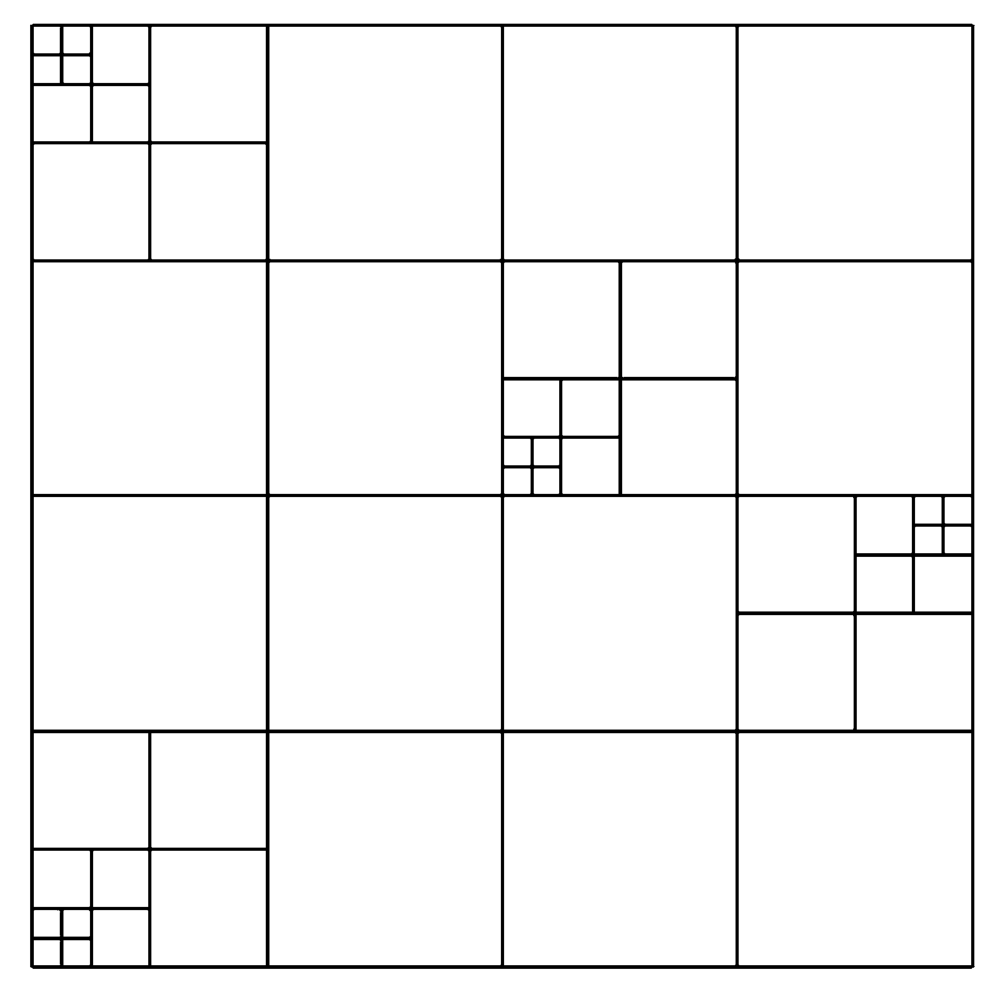
\includegraphics[width=0.9\textwidth]{imgs/figura5.png}
\caption{Malha non-graded para teste de Poisson}
\end{figure}
\end{column}
\end{columns}
\end{frame}

\begin{frame}{Resultados - Polinômios de 2º Grau}
\begin{table}
\centering
\caption{Erros com interpolações de 2º grau}
\begin{tabular}{ccccc}
\toprule
$h$ & $\|u-u_h\|_{L_\infty}$ & EOC & $\|\nabla u-\nabla u_h\|_{L_\infty}$ & EOC \\
\midrule
$\pi/32$ & 2.68e-2 & -- & 2.57e-2 & -- \\
$\pi/64$ & 6.08e-3 & 2.1 & 1.07e-2 & 1.3 \\
$\pi/128$ & 1.15e-3 & 2.3 & 3.18e-3 & 1.5 \\
$\pi/256$ & 2.39e-4 & 2.3 & 1.03e-3 & 1.5 \\
\bottomrule
\end{tabular}
\end{table}

\begin{itemize}
\item 2ª ordem para a solução $u_h$
\item Ordem reduzida (~1.5) para o gradiente $\nabla u_h$
\end{itemize}
\end{frame}

\begin{frame}{Resultados - Polinômios de 3º Grau}
\begin{table}
\centering
\caption{Erros com interpolações de 3º grau}
\begin{tabular}{ccccc}
\toprule
$h$ & $\|u-u_h\|_{L_\infty}$ & EOC & $\|\nabla u-\nabla u_h\|_{L_\infty}$ & EOC \\
\midrule
$\pi/32$ & 1.08e-2 & -- & 7.01e-3 & -- \\
$\pi/64$ & 1.80e-3 & 2.6 & 2.36e-3 & 1.6 \\
$\pi/128$ & 3.18e-4 & 2.5 & 6.96e-4 & 1.7 \\
$\pi/256$ & 7.65e-5 & 2.4 & 1.70e-4 & 1.8 \\
\bottomrule
\end{tabular}
\end{table}

\begin{itemize}
\item Melhora na ordem de convergência
\item 2ª ordem para solução e gradiente com polinômios de ordem superior
\end{itemize}
\end{frame}

\begin{frame}{Análise do Sistema Linear}
\begin{table}
\centering
\caption{Números de condição dos sistemas lineares}
\begin{tabular}{cccc}
\toprule
$h$ & Uniform grid & Batty [12] & Nosso método \\
\midrule
$\pi/32$ & 4.205e+01 & 7.171e+01 & 1.116e+03 \\
$\pi/64$ & 1.682e+02 & 2.815e+02 & 6.318e+03 \\
$\pi/128$ & 6.728e+02 & 1.193e+03 & 3.297e+04 \\
$\pi/256$ & 2.691e+03 & 4.713e+03 & 1.432e+05 \\
\bottomrule
\end{tabular}
\end{table}

\begin{itemize}
\item Números de condição ~32× maiores que Batty [12]
\item Escala com $\kappa(A) \approx 23/h^2$
\item Preenchimento (fill-in) decrescente com refinamento
\end{itemize}
\end{frame}

\begin{frame}{Conclusões Parciais}
\begin{block}{Vantagens do Método Proposto}
\begin{itemize}
\item \textbf{Robusto}: lida com malhas gerais hierárquicas
\item \textbf{Flexível}: não requer interpolações geométricas específicas
\item \textbf{Preciso}: mantém ordem de convergência esperada
\item \textbf{Generalizável}: extensão direta para 3D e dimensões superiores
\item \textbf{Eficiente}: computações locais, possibilidade de cache
\end{itemize}
\end{block}
\end{frame}
%----------------------------------------------------------------------------------------------------------------------	

\end{document}
%_______________________________________________________________________________________________________________________
